\documentclass[10t, a4paper, oneside]{ctexbook}
\usepackage{amsmath, amsthm, amssymb, bm, float,graphicx, geometry,hyperref, mathrsfs,forest,tikz}
\geometry{left = 2.54cm, right = 2.54cm, top = 3.18cm, bottom = 3.18cm}

\title{{\Huge{\textbf{数学建模课程笔记}}}}
\author{yangmei}
\date{\today}
\linespread{1.5}
\newtheorem{theorem}{定理}[section]
\newtheorem{definition}[theorem]{定义}
\newtheorem{lemma}[theorem]{引理}
\newtheorem{corollary}[theorem]{推论}
\newtheorem{example}[theorem]{例}
\newtheorem{proposition}[theorem]{命题}

\begin{document}

\maketitle

%\pagenumbering{roman}
%\setcounter{page}{1}

%\begin{center}
%    \Huge\textbf{前言}
%\end{center}~\

%这是笔记的前言部分. 
%~\\


\newpage
\pagenumbering{Roman}
\setcounter{page}{1}
\tableofcontents
\newpage
\setcounter{page}{1}
\pagenumbering{arabic}
 
\chapter{Secret Sharing}
\section{秘密共享}

Secret Sharing: 将秘密分成若干份,分发给不同的用户。用户特定子集共同提供各自的份额,才能重构初始秘密。

Treshold Scheme$(t,n)$ :在 $n$ 人之间共享秘密,其中任意 $t\le n$ 个人可求出秘密,任意 $t-1$ 个人无法求出秘密。
\section{Combinatorial Mathematics}
问题:
Eleven scientists are working on a secret project. They wish to lock up the documents in a cabinet so that the cabinet can be opened if and only if six or more of the scientists are present. What is the smallest number of locks needed? What is the smallest number of keys to the locks each scientist must carry?

采用组合数学的方法:
“少数”与“多数”:
\begin{enumerate}
    \item 设相关人共有 $2n+1$ 个,任意 $n$ 人组成的“少数”团体不能打开安全门,任意 $n+1$ 人组成的“多数”团体可以打开安全门  
    \item 两个不同的“少数”团体联合必包含某个多数团体  
    \item 任一“少数”团体和不属该团体的任一人联合可成为多数团体        
\end{enumerate}
锁与钥匙:
\begin{enumerate}
    \item 安全门上至少需要$\binom{2n+1}n$ 把锁 $\binom{11}5=462$
    \subitem 任一“少数”团体至少有一把锁不能打开
    \subitem 任意两个 少数"各不相同
    \item 每个人至少需要$\binom{2n}n$把钥匙 $\binom{10}5 = 252$
    每个人需拥有他所不属于的所有少数" 团体所打不开的锁的钥匙 
\end{enumerate}

用数学上集合的语言来表述: 给锁编号$1,2,\cdots,l$, 打开所有门的钥匙的全集即为 $K = {1,2,\cdots,l}$,任意第$i$人拥有的钥匙集合为$S_i$,则满足:

(1) $S_{i_1} \cup S_{i_2}\cup \cdots\cup S_{i_n} \subset K/k_i$\par
(2) $S_{i_1} \cup S_{i_2}\cup \cdots \cup S_{i_n}\cup S_{i_{n+1}} = K$
 
则有:
\begin{enumerate}
    \item 那么对于不同的 $n$ 的并,所对应的 $k_i$ 不同,任意一个 $k_i$ 必有一族 $\{i_1,i_2,\cdots i_n\}$ 与之对应 则 $k_i\in K$ 共有 $C_{2n+1}^n$ 个
    \item $k_i \in S_{i_{n+1}}$,这样的 $k_i$ 有 $C_{2n+1}^{n+1}$ 个
\end{enumerate} 



\section{Shamir's Threshold Scheme}

\subsection{Lagrange Polynomial interpolation} 

\begin{theorem}
Given $k$ points in the 2-dimensional plane $(x_1 y_1) \cdots (x_k, y_k)$. 
with distinct $x_i$'s , there is one and only one polynomial $q(x)$ of degree $k - 1$ such that $q(x_i) =y_i$ for all $x_i$.        
\end{theorem}

设多项式 $q(x) = a_0 + a_1 x + a_2 x^2 + \cdots+ a_{k-1} x^{k-1}, deg(q) = k-1$,  利用$k-1$组值求得$q(x)$的各项系数  
系数矩阵:

$$\begin{vmatrix}
1 & x_1 & x_1^2 & \cdots & x_1^{k-1} \\
1 & x_2 & x_2^2 & \cdots & x_2^{k-1} \\
\vdots & \vdots & \vdots & \ddots & \vdots \\
1 & x_k & x_k^2 & \cdots & x_k^{k-1} \\
\end{vmatrix} \neq 0$$

这是一个Vandermode行列式 

\subsection{Shamir 门限机制 $(t,n)$}

任选 $t-1$ 个整数 $x_1,x_2,\cdots,x_{t-1}$ 和 n 个互不相同的整数 $c_1,c_2,\cdots,c_n$ 。
素数 $p>n+1$求 $b_j\equiv(K+c_jx_1+c_j^2x_2+\cdots+c_j^{t-1}x_{t-1})\left({\mathrm{mod}}p\right),j=1,\cdots,n$ 其
中 $K\in\mathbb{Z}$ 为秘密

$$f(c)=K+x_1c+x_2c^2+\cdots+x_{t-1}c^{t-1},b_j\equiv f(c_j)({\mathrm{mod}}p),j=1,\cdots,n$$

将秘密份额$\left(c_j,b_j\right)$告知第 $_j$ 人

\begin{proof}{证明Shamir 门限机制的合理性}
 
    (1)若 $t$ 个人 $j_1,\cdots,j_t$ 共享秘密份额 $(c_{j_i},b_{j_i}),i=1,\cdots,t$\\
    方程组 $b_i\equiv\left(K+c_{j_i}x_1+c_{j_i}^2x_2+\cdots+c_{j_i}^{t-1}x_{t-1}\right)\left({\mathrm{mod}}p\right),i=1,\cdots,t$ 在模 $p$ 意义下有唯一解
    由于系数矩阵为
    $$\begin{vmatrix}1&c_1&c_1^2&\cdots&c_1^{t-1}\\1&c_2&c_2^2&\cdots&c_2^{t-1}\\\vdots&\vdots&\vdots&\vdots&\vdots\\1&c_{t-1}&c_{t-1}^2&\cdots&c_{t-1}^{t-1}\\1&c_t&c_t^2&\cdots&c_t^{t-1}\end{vmatrix}\neq 0$$
    其行列式为Vandermode行列式,即$det = \prod_{i = 1}^{k-1} (c_i-c_{i+1})$,因此$det \neq 0$同时$rank(row) = rank(column)$,方程有唯一解。

    (2)若 $t-1$ 个人 $j_1,\cdots,j_{t-1}$共享秘密份额 $(c_{j_i},b_{j_i}),i=1,\cdots,t-1$\\
    方程组 $b_{j_i}\equiv(K+c_{j_i}x_1+c_{j_j}^2x_2+\cdots+c_{j_i}^{t-1}x_{t-1})({\mathrm{mod}}p),i=1,\cdots,t-1$ 
    N
    含 $t-1$ 个方程,$t$ 个未知数,在模 $p$ 意义下有无穷多组解
    
\end{proof}
\section{Asmuth-Bloom's Threshold Scheme}
\subsection{中国剩余定理}
\begin{definition}[逆]
    设 $a,b$ 为整数,$m$ 为正整数,若 $ab\equiv 1(\mod m)$,则称 $a$ 模 $m$ 可逆,且 $b$ 是 $a$ 在模 $m$ 意义下的逆元,记为 $a^{-1}(mod m)$    
\end{definition}
$a$对模$m$可逆的$\Leftrightarrow (a,m) = 1$,即$a$与$m$互质

\begin{example}[大衍求一术求逆元]

    \begin{figure}[H]
        \centering
        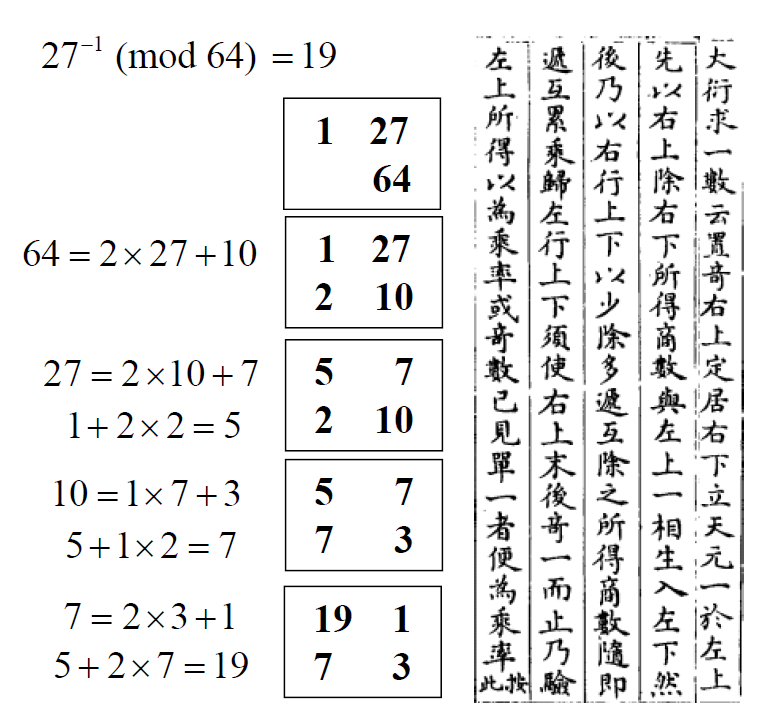
\includegraphics[width=8cm]{assets/大衍求一术.png}
    \end{figure}

\end{example}
\begin{definition}[一次同余方程]
    形如 $ax\equiv b(\mod m)$ 的方程,其中 $a,b,m$ 为整数,$m>0$。
\end{definition}

\begin{theorem}[线性同余方程有解和唯一]    
(1) 当且仅当 $gcd(a,m)|b$ 时,线性同余方程有解。\\
(2)当 $gcd(a,m)=1$ 时,方程的解为 $a^{-1}b$,且小于 $m$的非负整数解唯一。\\
其中 $a^{-1}$ 是 $a$ 在模 $m$ 意义下的逆元。      
\end{theorem}

\begin{theorem}[中国剩余定理(数论)]
    设 $m_1,m_2,\cdots,m_k$ 为两两互质的正整数,$a_1,a_2,\cdots,a_k$ 为任意整数,记$M = m_1m_2\cdots m_k$,则一次同余方程组

    $$
    \begin{cases}
    x\equiv a_1(\mod m_1)\\
    x\equiv a_2(\mod m_2)\\
    \vdots\\
    x\equiv a_k(\mod m_k)\\
    \end{cases}
    $$

    (1)有小于 $M$ 的唯一正整数解$x=M_1M_1^{-1}a_1+M_2M_2^{-1}a_2+\cdots+M_kM_k^{-1}a_k(\mod M)$,其中$M_i=M/m_i$,$M_i^{-1}$是$M_i$在模$m_i$意义下的逆元。 
    
    (2)对任意 $l\in\mathbb{Z}$,$x+l\cdot m$也是同余方程组的解.
\end{theorem}
\begin{theorem}[中国剩余定理(代数多项式)]
    设 ${f_i(x)|i = 1,\cdot,n}$ 是两两互素的多项式, $a_1(x), a_2(x),\cdots,a_n(x)$ 是 $n$ 个多项式,则存在多项式 $g(x)$,$q_i(x)(i= 1,2\cdots, n)$,使得 $g(x) = f_i(x)q_i(x) + a_i(x)$ 对一切 $i$ 成立。   
\end{theorem}

\begin{example}[物不知数]
    $$
    \begin{cases}
    &x\equiv2(\mathrm{mod}3)\quad N_1=5\cdot7=35\quad N_1^{-1}(\mathrm{mod}3)=2\\
    &x\equiv3(\mathrm{mod}5)\quad N_2=3\cdot7=21\quad N_2^{-1}(\mathrm{mod}5)=1\\
    &x\equiv2(\mathrm{mod}7)\quad N_3=3\cdot5=15\quad N_3^{-1}(\mathrm{mod}7)=1
    \end{cases}
    $$
    $$\begin{aligned}m=3\cdot5\cdot7=105&\quad35\cdot2\cdot2+21\cdot1\cdot3+15\cdot1\cdot2=233\\&\quad x=23\equiv233\mathrm{~(mod~}105)\end{aligned}$$
\end{example}  

\subsection{Asmuth-Bloom门限机制 $(t,n)$}

设秘密为 $K$\\
(1)选取整数 $p$ 与 $m_1,\cdots,m_n$\\
$p>K$ 且 $p$ 与 $m_j,1\leq j\leq n$ 互素,$m_1<\cdots<m_n$ 且 $m_1,\cdots,m_n$ 两两互素 \\
$$\frac{m_1\cdots m_t}{m_{n-t+2}\cdots m_n}>p$$
即为$m_1,\cdots,m_n$ 中任意 $t$ 个数的乘积与任意 $t-1$ 个数的乘积之比大于$p$\\
(2)令 $K^{\prime}=K+r\cdot p$,其中 $r\in\mathbb{N}$ 满足\par
(i)$0\leq r\leq\frac{m_1\cdots m_t}p-1$\par
(ii)$K^{\prime}=K+r\cdot p\leq K+m_1\cdots m_t-p<m_1\cdots m_t$\\
再令$k_j\equiv K^{\prime}({\mathrm{mod}}m_j),1\leq j\leq n$, 将秘密份额$(k_j,m_j)$告知第 $j$ 人

\begin{proof}{证明Asmuth-Bloom门限机制的合理性}\\
    $k_j\equiv K'({\mathrm{mod}}m_j),1\leq j\leq n$ ,因此$K'$满足的方程: $K'\equiv k_j({\mathrm{mod}}m_j),1\leq j\leq n$\\
    $K'=K+r\cdot p<m_1\cdots m_t$ ,$K'$对$p$取模求出$K$: $K\equiv K'(\text{mod }p)$\\
    一次同余方程组 (I) $x\equiv k_j\left({\mathrm{mod}}m_j\right),1\leq j\leq n$ 有唯一的小于 $m_1\cdots m_n$ 的非负整数解 $K'$\par
    (1)若 $t$ 个人 $j_1,\cdots,j_t$ 共享秘密份额 $\left(k_{j_i},m_{j_i}\right),i=1,\cdots,t$\\
    一次同余方程组 (II) $x\equiv k_{j_i}({\mathrm{mod}}m_{j_i}),\:i=1,\cdots,t$ 有唯一的小于 $m_{j_1}\cdots m_{j_t}$ 的正整数解 $X$\\
    $K'$也为方程(II) 的解,且 $K^{\prime}<m_1\cdots m_t<m_{j_1}\cdots m_{j_t}$ 。由中国剩余定理,解的唯一性有 $K'= X$ 
    \begin{figure}[H]
        \centering
        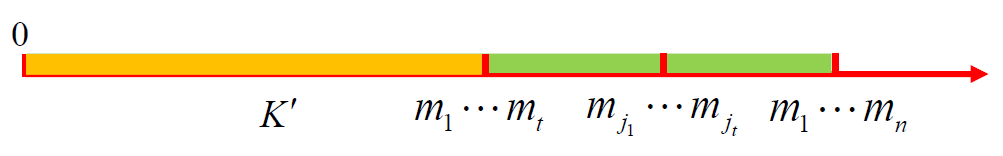
\includegraphics[width=8cm]{assets/方程ⅡK'值所在区间.png}
    \end{figure}
    (2) 若 $t-1$ 个人 $j_1,\cdots,j_{t-1}$ 共享秘密份额$\left(k_{j_i},m_{j_i}\right),i=1,\cdots,t-1$\\
    一次同余方程组 (III) $x\equiv k_{j_i}({\mathrm{mod}}m_{j_i}),\:i=1,\cdots,t-1$ 有唯一的小于$m_{j_1}\cdots m_{j_{t-1}}$的正整数解$Y$\\
    $Y+l\cdot m_{j_1}\cdots m_{j_{t-1}} < \frac{1+l}{p}*m_{j_1}m_{j_2}\cdots m_{j_{t}},l\in\mathbb{Z}$ 均为方程组 (III) 的解,  $K'$ 为这些解中的某一个, $K'$ 的限制条件仅有 $K' < m_1 m_2\cdots m_t$,因此 $K'$ 不能唯一确定 
    \begin{figure}[H]
        \centering
        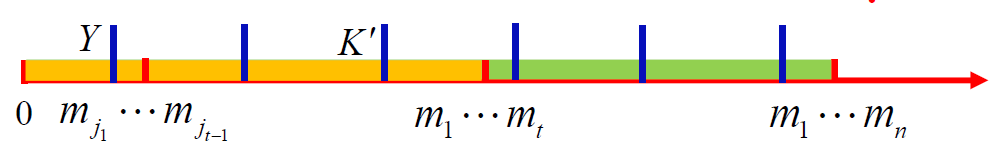
\includegraphics[width=8cm]{assets/方程ⅢK'值所在区间.png}
    \end{figure}
\end{proof}

\noindent(1)Liu, C.L. Introduction to Combinatorial Mathematics. McGraw-Hill,1968\\
(2) Shamir A. How to share a secret. Communications of the ACM, 1979, 22(11): 612-613.\\
(3) Asmuth AC, Bloom J. A modular approach to key safeguarding. IEEE Transactions on Information Theory, 29, 208-210, 1983.\\

\newpage
\chapter{Page Rank}
\section{网页重要度}
\noindent\textbf{网页重要度的原则与假设}\\
某网页重要,是因为有重要的网页链接到它,对任一网页A,确定一数值为其重要度,作为网页排序的依据
链接到网页A的所有网页对网页A的重要度均有贡献,贡献大小与这些网页自身的重要度有关
\begin{enumerate}	
    \item (传递性)重要度大的网页链接到网页A时对网页A的重要度的贡献比重要度小的网页链接到网页A时对网页A的重要度的贡献大:某网页对其它网页重要度的贡献之和等于它的重要度
    \item (等效性)网页对它所链接的每个网页的重要度的贡献相等:某网页对其它网页的重要度贡献与它所链接的网页数量呈反比
    \item (叠加性)链接到网页A的网页越多,网页A越重要:网页A的重要度是所有链接到A的网页对网页A的重要度的贡献之和
    \item (无关性)网页链接其它网页的多少,与其本身的重要度无关
\end{enumerate}	
\noindent\textbf{网页链接图}
\begin{definition}[网页链接图]
    互联网中网页之间的链接关系可用图表示,称为网络链接图。
    \begin{enumerate}
        \item[顶点]网页 $\nu_1,\nu_2,\cdots,\nu_n$ 
        \item[弧]网页间的链接关系,即若网页$\nu_i$上有链接指向网页$\nu_j$,则网络链接图中有一条以$\nu_i$为起点,$\nu_j$ 为终点的弧
        \item[出度]以某顶点为起点的弧的总数,即该网页链接的网页数量
    \end{enumerate}    
\end{definition}
\noindent\textbf{网页重要度的矩阵表示}\\
网页 $\nu_i$ 的重要度记为 $x_i$ 出度记为$q_i$
\begin{enumerate}
    \item[传递性]网页 $\nu_i$ 对其它网页重要度贡献之和为 $x_i$
    \item[等效性]网页 $\nu_i$ 对它链接的$q_i$ 个网页中的任一个的重要度贡献为$\frac{x_i}{q_i}$
    \item[叠加性]若链接到网页$\nu_j$的网页有$\nu_{j_1},\nu_{j_2},\cdots,\nu_{j_k}$,则
        $$x_j=\frac{x_{j_1}}{q_{j_1}}+\frac{x_{j_2}}{q_{j_2}}+\cdots+\frac{x_{j_k}}{q_{j_k}}$$
\end{enumerate} 

\noindent 记$p_{ij}$为网页$v_i$到$v_j$的链接概率,即$v_i$链接到$v_j$的概率,有
$$p_{ij}=\begin{cases}
\frac{1}{q_j},&\text{若}v_j\text{链接到}v_i\\
0,&\text{若}v_j\text{不链接到}v_i
\end{cases}$$
所以,上式改写为
$$x_i=\sum_{j=1}^np_{ij}x_j$$
记矩阵$\mathbf{P}=(p_{ij})_{n\times n}$为初始链接矩阵(网页$v_j$的出度列向量$\mathbf{p_j} = (p_{1j},p_{2j,\cdots,p_{nj}})^T$,$\mathbf{x}=(x_1,x_2,\cdots,x_n)^T$为网页重要度向量,
则$\mathbf{x}$为线性方程方程$\mathbf{x}=\mathbf{P}\mathbf{x}$的解。
\begin{equation}
    \mathbf{x}=\mathbf{P}\mathbf{x}
\end{equation}
\noindent(1)$\mathbf{x}$是$\mathbf{P}$的特征向量,对应的特征值为1。\\
(2)$\text{Rank}(\mathbf{I}-\mathbf{P})<n$ 由于$\mathbf{1}^T(\mathbf{I}-\mathbf{P}) = \mathbf{0}$,即说明其行向量线性相关,因此方程(2.1)有非零解\\
(3)方程(2.1)一定有非零解吗,即重要度向量$\mathbf{x}$一定存在吗,以及存在一定唯一吗,这个问题之后分析。
\begin{example}[链接矩阵与重要度向量的求解]
    \begin{figure}[H]
        \centering
        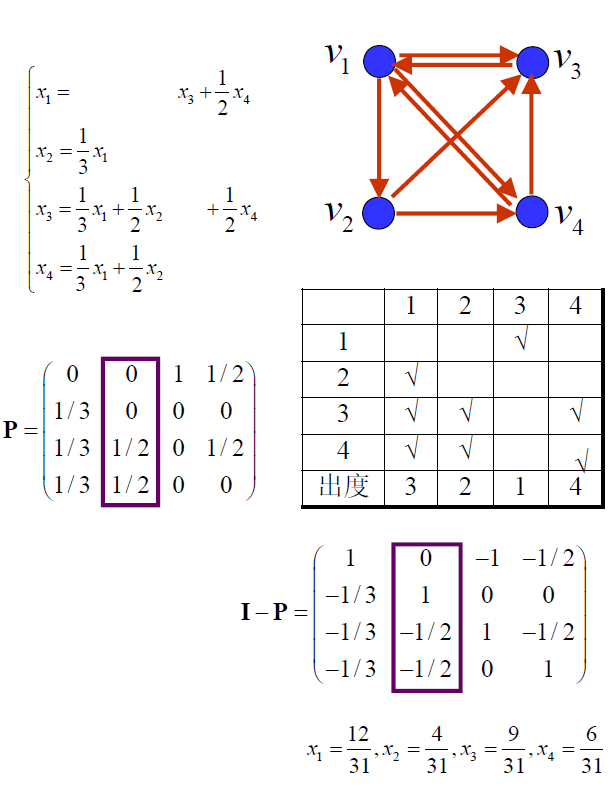
\includegraphics[width=8cm]{assets/网页重要度例题.png}
    \end{figure}
\end{example}
\section{随机矩阵}
\begin{definition}
\noindent 各行 (列) 元素之和均为 1 的非负方阵称为行 (列) 随机矩阵 (row(column) stochastic matrix)\\
各行与各列元素之和均为 1 的非负方阵称为双随机矩阵 ( doubly stochastic matrix )
\end{definition}
\begin{proposition}
    随机矩阵一定存在特征值为1对应的特征向量  
\end{proposition}
\begin{proof}
    上文已经简单地从行秩的角度说明了$(\mathbf{P}-\mathbf{I})\mathbf{x} = 0$有非零解,下面以列随机矩阵从行列式的角度证明$det({\mathbf{P}-\mathbf{I}}
    ) = 0$,从而证明行列式有非零解。

    $$\begin{aligned}
        &det({\mathbf{P}-\mathbf{I}}) = 
        \begin{vmatrix}
            &p_{11}-1 & p_{12} &\cdots& p_{1n}\\
            &p_{21} &p_{22}-1&\cdots&p_{2n}\\
            &\vdots&\vdots&\ddots&\vdots\\
            &p_{n1}&p_{n2}&\cdots&p_{nn}-1
        \end{vmatrix}\\
        &=\begin{vmatrix}
            &\sum_{i=1}^np_{i1}-1 & \sum_{i=1}^np_{i2} &\cdots& \sum_{i=1}^np_{in}\\
            &p_{21} &p_{22}-1&\cdots&p_{2n}\\
            &\vdots&\vdots&\ddots&\vdots\\
            &p_{n1}&p_{n2}&\cdots&p_{nn}-1
        \end{vmatrix}
        =\begin{vmatrix}
            &0& 0 &\cdots& 0\\
            &p_{21} &p_{22}-1&\cdots&p_{2n}\\
            &\vdots&\vdots&\ddots&\vdots\\
            &p_{n1}&p_{n2}&\cdots&p_{nn}-1
        \end{vmatrix} = 0
    \end{aligned}$$
\end{proof}

\begin{theorem}[随机矩阵的模最大特征值]
    任一随机矩阵的模最大特征值为 1   
\end{theorem}
\begin{proof}
    设 $\lambda$ 是行随机矩阵 $\mathbf{P}=(p_{ij})_{n\times n}$ 的特征值,非零向量 $\mathbf{X} = ( x_1, \cdots , x_n) ^{\mathrm{T} }$ 为属于特征值 $\lambda$ 的特征向量。设$|x_i|=\max_{1\leq j\leq n}|x_j|>0$\\
    由 $\mathbf{PX}=\lambda\mathbf{X}$,可得 $\lambda x_i=\sum_{j=1}^np_{ij}x_j$。 两边取模,$|\lambda\|x_i|=|\lambda x_i|=\left|\sum_{i=1}^np_{ij}.x_j\right|\leq\sum_{i=1}^n|p_{ij}\|x_j|\leq|x_i|\sum_{i=1}^n|p_{ij}|=|x_i|$, 即$|\lambda|\leq1$
\end{proof}

\section{链接矩阵}
\noindent\textbf{链接矩阵的基本性质}\\
(1)链接矩阵 $\mathbf{P}$ 的每列元素之和为 1 ,为列随机矩阵\\
(2)链接矩阵 $\mathbf{P}$ 一定存在特征值为$1$的非零特征向量\\
(3)  $\mathbf{1}^T \mathbf{P} = \mathbf{1}^T$

\subsection{悬挂网页修正}
\noindent 悬挂网页(dangling link): 若某网页不链接任意其它网页\\
悬挂网页修正:将链接矩阵 $\mathbf{P}$ 中对应列的所有元素由 $0$ 修改为 $\frac{1}{n}$,得到修正链接矩阵$\overline{\mathbf{P}}$\\
$$\overline{\mathbf{P}}=\mathbf{P}+\frac1n\mathbf{1}\mathbf{d}^\mathrm{T}$$
其中 $\mathbf{1}$ 为分量全为 $0$ 的列向量。
\begin{example}[悬挂网页修正]
    \begin{figure}[H]
        \centering
        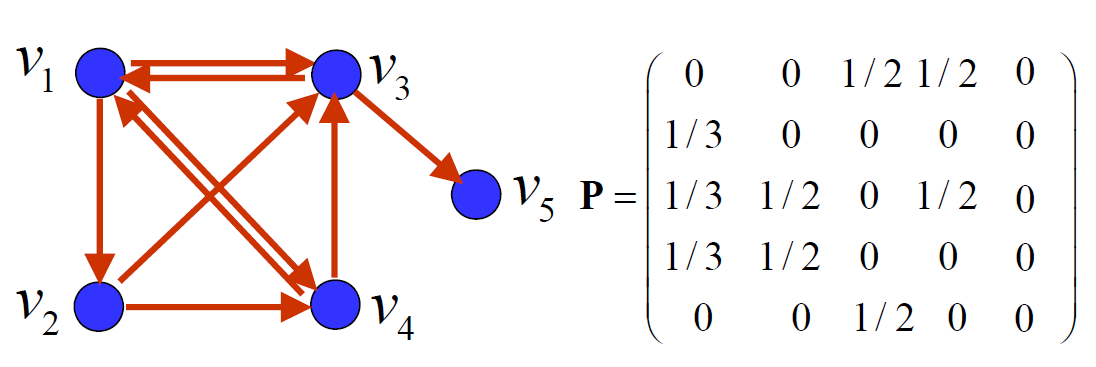
\includegraphics[width = 8cm]{assets/修正矩阵-原矩阵.png}
        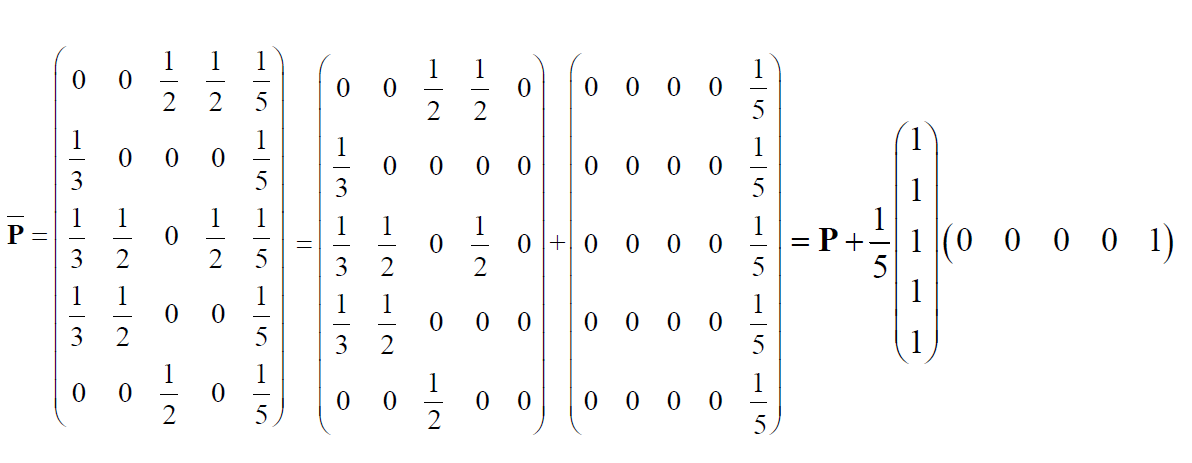
\includegraphics[width=8cm]{assets/修正矩阵-修正后矩阵.png}       
    \end{figure}
\end{example}
\subsection{多解修正}
若 P 有两个属于特征值 1 的线性无关的特征向量重要度向量排序不唯一\\
\begin{figure}[H]
    \centering
    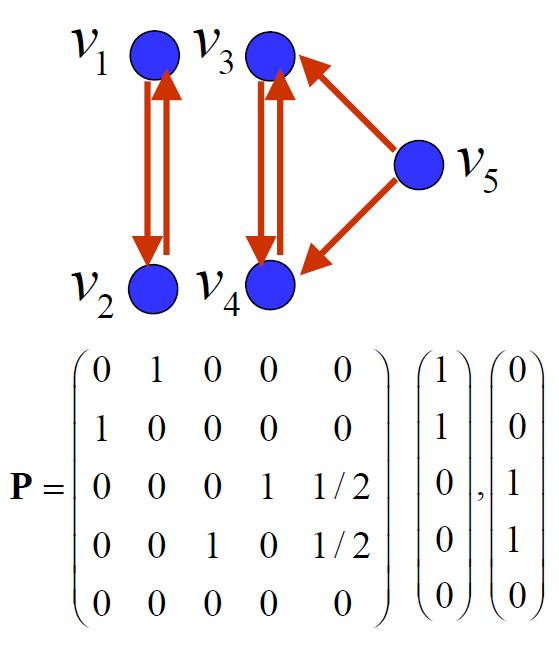
\includegraphics[width = 4cm,height = 4cm]{assets/两个特征向量的修正矩阵.png}
    \caption{修正矩阵 $\overline{\mathbf{P}}$ 具有两个特征值为一的特征向量(重要度向量)}  
\end{figure}

\noindent 将 $\overline{\mathbf{P}}$修改为最终的链接矩阵,修正方法:

$$\overline{\overline{\mathbf{P}}}=\alpha\overline{\mathbf{P}}+(1-\alpha)\frac{1}{n}{\mathbf{-}}\mathbf{11}^{\mathrm{T}}$$ 

其中参数 $\alpha=0.85$

$\overline{\overline{\mathbf{P}}}$ 为完全正矩阵 (totally positive matrix) 与列随机矩阵:

$$\mathbf{1} ^{\mathrm{T} }\overline{\overline{\mathbf{P}}} = \alpha\mathbf{1} ^{\mathrm{T} }\mathbf{P} + ( 1- \alpha) \mathbf{- } \mathbf{1} ^{\mathrm{T} }\mathbf{1} \mathbf{1} ^{\mathrm{T} }= \alpha\mathbf{1} ^{\mathrm{T} }+ ( 1- \alpha) \mathbf{1} ^{\mathrm{T} }= \mathbf{1} ^{\mathrm{T} }$$

\begin{figure}[H]
    \centering
    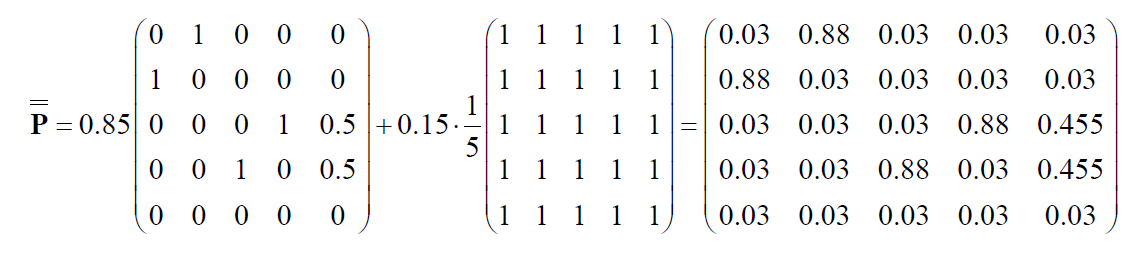
\includegraphics[width = 8cm]{assets/多解修正.png}
    \caption{多解修正}
\end{figure}

\subsection{重要度向量的存在唯一性}
根据随机矩阵存在特征值为1的特征向量,因此链接矩阵的重要度向量一定存在。下证它的唯一性。
\begin{lemma}
    完全正、列随机矩阵属于特征值的特征向量分量之和不为0。
\end{lemma}
\begin{proof}
    设$\mathbf{x}$是完全正、列随机矩阵 $\mathbf{P}$ 的属于特征值1的特征向量,则$x_i=\sum\limits_{j=1}^n\overline{\overline{p}}_{ij}x_j$
        
        若$\sum\limits_{i=1}^nx_i=0$,则$\mathbf{x}$的分量有正有负,故
        
        $$|x_i|=|\sum\limits_{j=1}^n\overline{\overline{p}}_{ij}x_j|<\sum\limits_{j=1}^n\overline{\overline{p}}_{ij}|x_i|$$

        故而

        $$\sum\limits_{i=1}^n|x_i|<\sum\limits_{i=1}^n\sum\limits_{j=1}^n\overline{\overline{p}}_{ij}|x_j|=\sum\limits_{j=1}^n\sum\limits_{i=1}^n\overline{\overline{p}}_{ij}|x_j|=\sum\limits_{j=1}^n(|x_j|\sum\limits_{i=1}^n\overline{\overline{p}}_{ij})=\sum\limits_{j=1}^n|x_j|$$

        矛盾。
\end{proof}
\begin{proposition}
    完全正、列随机矩阵仅有 1 个属于特征值 1 的线性无关的特征向量。
\end{proposition}
\begin{proof}
    
    设$\mathbf{v}=(v_1,v_2,\cdots,v_n)^T, \mathbf{w}=(w_1,w_2,\cdots,w_n)^T$是完全正、列随机矩阵$\mathbf{P}$的两个属于特征值1的线性无关的特征向量。令$x_i = -\frac{W}{V}v_i+w_i, i = 1,2,\cdots,n$,其中$W=\sum_{i=1}^nw_i, V=\sum_{i=1}^nv_i\neq 0$.
    
    首先若向量 $\mathbf{x} = (x_1,x_2,\cdots,x_n)$ 是 $\mathbf{P}$ 的特征值为 $\lambda$ 的特征向量 $\Leftrightarrow \forall i, \sum\limits_{j=1}^n p_{ij}x_j=\lambda x_i$,根据特征向量的定义即可证得。

    由$\mathbf{v}$和$\mathbf{w}$线性无关,且
    $$\sum\limits_{j=1}^n p_{ij}x_j=\sum\limits_{j=i}^n p_{ij}(-\frac{W}{V}v_j+w_j)=-\frac{W}{V} p_{ij}v_j+\sum\limits_{j=i}^n p_{ij}w_j=-\frac{W}{V}v_i+w_i=x_i$$

    可知 $\mathbf{x}=(x_1,\cdots,x_n)$为 P 的属于特征值 1 的特征向量
   
    又有
    $$\sum\limits_{i=1}^nx_i = \sum\limits_{i=1}^n(-\frac{W}{V}v_i+w_i) = -\frac{W}{V}\sum\limits_{i=1}^nv_i+\sum\limits_{i=1}^nw_i = -\frac{W}{V}V+W = 0$$

    即$\mathbf{x}$的分量之和为零。

    从而与上面的结论矛盾。
\end{proof}

\subsubsection{Perron—Frobenius定理}
\noindent\textbf{Perron定理}\\
若矩阵 $\mathbf{A}$是完全正矩阵,则\\
    (1) $\mathbf{A}$的模最大特征值唯一,且为正实数\\
    (2) 该特征值代数重数为1\\
    (3) 存在该特征值的一个特征向量,其分量全为正\\
\noindent\textbf{Perron—Frobenius定理}\\
若矩阵 $\mathbf{A}$是非负\textbf{不可约}(irreducible)矩阵,则\\
    (1) $\mathbf{A}$的模最大特征值为正实数\\
    (2) 该特征值代数重数为1\\
    (3) 存在该特征值的一个特征向量,其分量全为正
\begin{figure}[H]
    \centering
    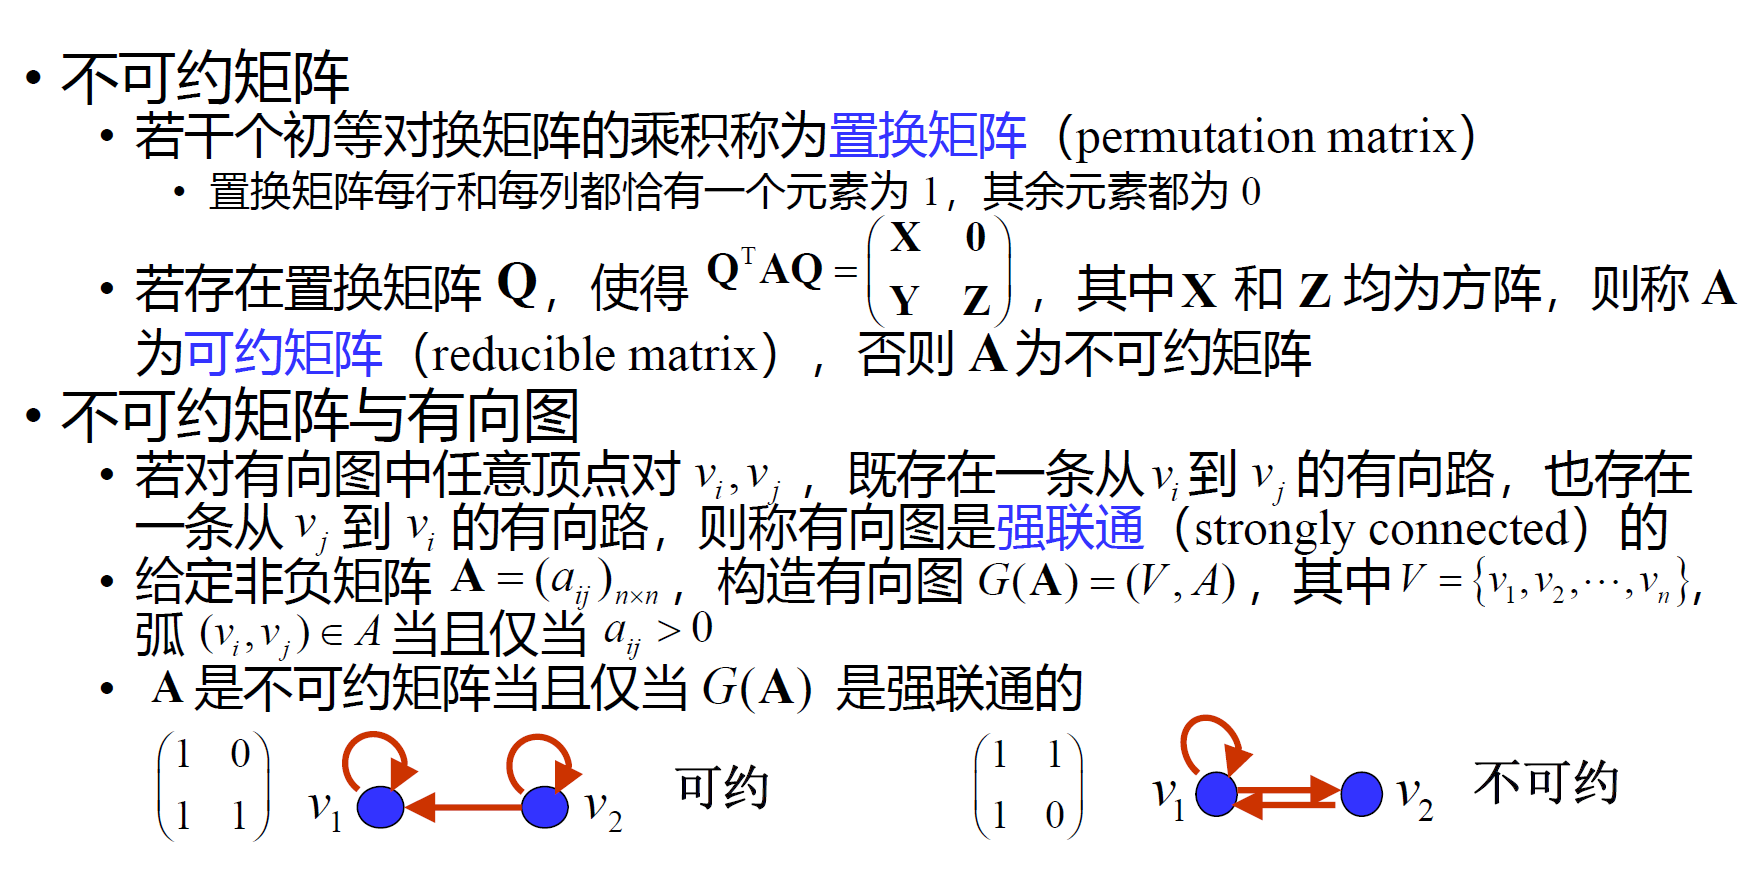
\includegraphics[width = 15cm]{assets/不可约矩阵.png}
    \caption{不可约矩阵简单介绍}
    
\end{figure}
\noindent\textbf{链接矩阵与重要度向量}\\
链接矩阵为\underline{完全正、列随机矩阵},模最大特征值为1,重要度向量\underline{唯一且分量全为正}.    
    
\section{矩阵计算}
\subsection{幂法迭代}

幂法是计算矩阵模最大特征值和对应的特征向量的一种迭代算法

任取初始向量$\mathbf{x}^{(0)}>0$,且$\sum\limits_{i=1}^nx_i^{(0)}=1$,

迭代计算$\mathbf{x}^{(k)}=\overline{\overline{\mathbf{P}}}\mathbf{x}^{(k-1)}$,直到$\mathbf{x}^{(k)}$收敛\\
迭代后的向量仍然向量之和为1:
$$\mathbf{1}^T\mathbf{x}^{(k)}=\mathbf{1}^T\overline{\overline{\mathbf{P}}}\mathbf{x}^{(k-1)}=\mathbf{1}^T\mathbf{x}^{(k-1)}=1$$

将$\overline{\mathbf{P}}=\mathbf{P}+\frac{1}{n}\mathbf{1}\mathbf{d}^T$, $\overline{\overline{\mathbf{P}}}=\alpha\overline{\mathbf{P}}+(1-\alpha)\frac{1}{n}\mathbf{1}\mathbf{1}^T$
两式带入迭代计算式中

$$\begin{aligned}
    \mathbf{x}^{(k)}&=\overline{\overline{\mathbf{P}}}\mathbf{x}^{(k-1)}\\
    &=\alpha\overline{\mathbf{P}}\mathbf{x}^{(k-1)}+(1-\alpha)\frac{1}{n}\mathbf{1}\mathbf{1}^T\mathbf{x}^{(k-1)}\\
    &=\alpha\overline{\mathbf{P}}\mathbf{x}^{(k-1)}+(1-\alpha)\frac{1}{n}\mathbf{1}\\
    &=\alpha(\mathbf{P}+\frac{1}{n}\mathbf{1}\mathbf{d}^T)\mathbf{x}^{(k-1)}+(1-\alpha)\frac{1}{n}\mathbf{1}\\
    &=\alpha\mathbf{P}\mathbf{x}^{(k-1)}+\alpha\frac{1}{n}\mathbf{1}\mathbf{d}^T\mathbf{x}^{(k-1)}+(1-\alpha)\frac{1}{n}\mathbf{1}\\
\end{aligned}$$

\subsection{完全正、列随机矩阵的幂法收敛性}
\begin{proof}
    记$\mathbf{V}$为满足$\mathbf{1}^T\mathbf{v}= 0 $的$n$维列向量$\mathbf{v}=\{v_1,v_2,\cdots,v_n\}$全体组成的集合。记$\|\mathbf{v}\|_1=\sum\limits_{i=1}^n|v_i|$(范数)\\
    对任意的$\mathbf{v}\in\mathbf{V}$,取$\mathbf{w}=\mathbf{P}\mathbf{v}$,下证:$\left\|\mathbf{w}\right\|_1\leq c\left\|\mathbf{v}\right\|_1$, 其中$c<1$

    \noindent 若$\mathbf{w}=0$,显然成立。\\
    若$\mathbf{w}\neq0$,记$\mathbf{w}=(w_1,w_2,\cdots,w_n)^T$,$e_i = \text{sgn}(w_i)$,则 $c=\max_{j}\left|\sum_{i=1}^{n}p_{ij}e_{i}\right|<\left|\sum_{i=1}^np_{ij}e_{i}\right|<1$ 
    $$\begin{aligned}
        \left\|\mathbf{w}\right\|_1
        &=\sum_{i=1}^n\left|\mathbf{w}_i\right|=\sum_{i=1}^ne_iw_i=\sum_{i=1}^ne_i\left(\sum_{j=1}^np_{ij}\nu_j\right)=\sum_{j=1}^nv_j\left(\sum_{i=1}^np_{ij}e_i\right)\\
        &\leq\sum_{j=1}^n\left|v_j\right|\left|\sum_{i=1}^np_{ij}e_i\right|\leq c\sum_{j=1}^n\left|\mathbf{v}_j\right|=c\left\|\mathbf{v}\right\|_1
    \end{aligned}$$
\end{proof}
\section{随机浏览}
\begin{definition}[随机浏览]
    按以下模式浏览互联网的网页
\begin{enumerate}
    \item 有时从当前网页的链接中随机打开一个网页
    \item 有时键入网址新建一个网页
    \item 从任一网页开始,充分长时间后,访问各网页的概率即为网页重要度
\end{enumerate}
\end{definition}
经过统计,随机打开网页的次数与键入网址新建网页的次数之比约为$5:1$,也即$\alpha=0.85$。

\begin{definition}[随机概率]
记事件 $\{X_m=j\}$ 为时刻 $m$ 访问网页 $v_j$,则$P\{X_m=i | X_{m-1}=j\}=p_{ij}$

若  $P\{X_m=j\}=x_j$,则$P\{X_{m}=i\}=\sum\limits_{j=1}^nP\{X_m=i | X_{m-1}=j\}P\{X_{m-1}=j\}=\sum\limits_{j=1}^np_{ij}x_j$

记 $\mathbf{x}^{(m)}=(P\{X_m=1\},P\{X_m=2\},\cdots,P\{X_m=n\})^T$,则有$\mathbf{x}^{(m)}=\overline{\overline{\mathbf{P}}}\mathbf{x}^{(m-1)}$
\end{definition}
\begin{definition}[随机过程]
随机过程是描述随机现象随时间推移而演化的一类数学模型。\\
在一族随机变量$\{X(t),t\in T\}$中$T$为参数集,$t$是参数。$\{X(t),t\in T\}$称为参数为$t$的随机变量。$T$为整数集的随机过程称为随机序列。
\end{definition}
\begin{definition}[Markov过程]
在已知目前的状态的条件下,它未来的演变不依赖于它以往的演变。\\
在随机序列$\{X(n),n=0,1,2,\cdots\}$中($X_n$有限或可列),对任意的$n\geq0$,有
$$P\{X_{n+1}=j | X_n=i,X_{n-1}=i_{n-1},\cdots,X_0=i_0\}=P\{X_{n+1}=j | X_n=i\}$$
\end{definition}
\newpage
\chapter{数论与组合模型}
\section{Nim Game}
现有$n$堆硬币,每堆数量一定。两人轮流取硬币,每次只能从其中一堆中取,且每次取至少一枚。取到最后一枚硬币的一方获胜。 
\subsection{位值制计数法}
选定进位制的基底 $b$ , 给定 $0,1,2,\cdots,b-1$共 $b$ 个数码。任何一个自然数$N$, 均可用某个以这些数码为系数的 $b$ 的多项式表示出来。
$$
\begin{aligned}N&=a_k\cdot b^k+a_{k-1}\cdot b^{k-1}+\cdots+a_1\cdot b+a_0\\&\Rightarrow\left(a_ka_{k-1}\cdots a_1a_0\right)_b,\:a_0,a_1,\cdots,a_k\in\left\{0,1,\cdots,b-1\right\}\end{aligned}
$$
\begin{proposition}
(1)任意数的 $b$ 进制表示是唯一的
\begin{proof}
    可以取模证明。 
\end{proof} 
(2)任意两个数的 $b$ 进制表示不同 
\begin{proof}
    根据(1)$0$的 $b$ 进制表示是唯一的用反证法证明。
\end{proof}
\end{proposition}
\subsection{Nim Game的必胜策略}
\subsubsection{Safe Combination 安全状态}
(1)安全状态:若无论对方如何取均不会获胜,或者无论对方如何取,己方下一次取后均可变为一个安全状态的,称为安全状态。

(2)不安全状态若对方至少存在一种获胜的取法,己方下一次取无法变为一个安全状态的,称为不安全状态。

必胜策略:己方取法使得下一状态为安全状态。
\subsubsection{二进制位和与安全状态}
\noindent\textbf{二进制与位和:}
将每堆硬币数表示为二进制。将所有二进制数的每一位数字分别求和,其尾数称为位和。

Write the number of the counters in each pile in the binary scale of notation,  and place these numbers in three horizontal lines so that the units are in the same vertical column. If then the sum of each column is 2 or 0 (i.e.congruent to 0, mood.2), the set of numbers forms a safecombination. 
\begin{theorem}[Basic Property]
    If a, b, c form a safe combination any two of the numbers determine the remaining one, that is, the system is closed.
    So it is for $n$ piles situation.
\end{theorem}
\begin{corollary}
    (1)只有一堆硬币时,位和不可能全为0\\
    (2)每次从某一堆中取若干枚硬币,该堆硬币的二进制数发生变化,且至少有一位位和发生变化。\\
\end{corollary} 
\noindent\textbf{位和和安全状态:}   
若所有位和均为 0 ,则当前状态为安全的,否则为不安全

\noindent(1)若当前状态安全,对任意取法,状态变为不安全

    只能从一堆中取,由于当其他$n-1$堆在给定时,能让这$n-1$堆直和第$n$堆变为安全状态的第$n$堆是唯一确定的,就是当前安全状态下要取走的这堆的数目,所以取走该堆的任意个硬币后,都不能达到安全状态。\\
(2)若当前状态不安全,存在一种取法,状态变为安全

    按自左至右的顺序确定第一个数字之和不为 0 的位,寻找该位数字为 1 的堆,从该堆中取走若干枚使得状态变为安全

\noindent\textbf{Nim Game 必胜情况与先后手的关系}\\
(1) 若初始状态不安全,先手必胜。若初始状态安全,后手必胜\\
(2) 必胜一方选择适当的取法,使取后状态对己方是安全的

因此先手必胜的概率可以从 Nim Game 随机开局时是否为不安全状态算出,即
$$P{\text{先手必胜}} = P{\text{开局为不安全状态}} = \frac{\text{不安全状态个数}}{\text{所有开局可能个数}}(\text{古典概型})$$

\section{伪币称重问题}
\noindent\textbf{伪币辨识}
12枚外观相同的硬币中有一枚是伪币,伪币质量与真币不同(偏轻或者偏重不知),能否用天平称量三次找出伪币,并说明伪币相对真币偏轻或偏重。其中天平一次称量只能比较两端质量大小,不能读出质量数值
\subsection{自适应方案}
硬币真伪的可能性共有$12\times2 = 24$种。每一种称量结果对应一种可能性,不同称量结果对应的可能性各不相同\\
\textbf{自适应与非自适应}
\begin{definition}
后一次称量依赖于之前称量结果的方案为自适应(adaptive)的,否则称为非自适应(non-adaptive)的。\\
\end{definition}
\textbf{Type Konwn 伪币称重的自适应方案}
\begin{figure}[H]
    \centering
    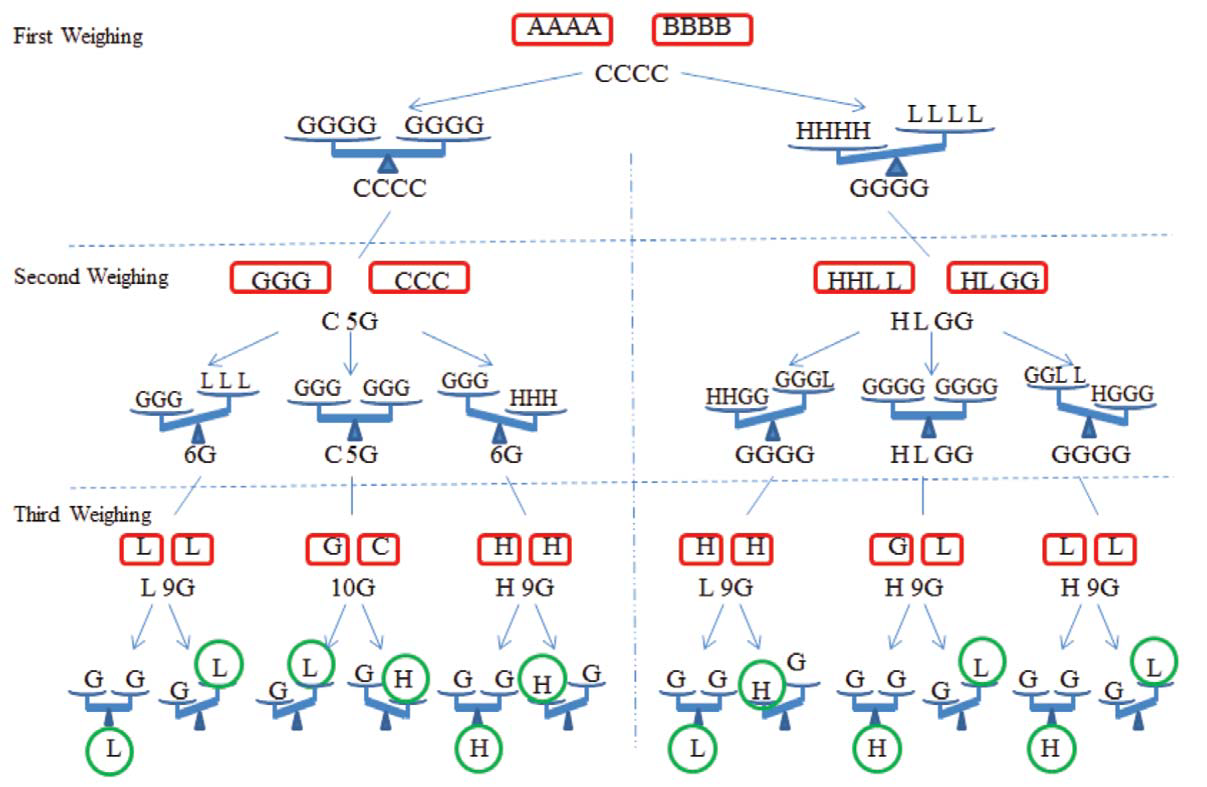
\includegraphics[width = 15cm]{assets/sequential_weighing_design.png}
    \caption{A sequential weighing design for c = 12 coins in w = 3 weighings with type konwn}
\end{figure}
自适应方案的核心在于:在每一次称重后,我们都需要把解答的空间缩小到原来的 1/3。
\subsection{非自适应方案}
\noindent{Type Konwn自适应最优方案}\\
若 $3\leq n\leq \frac{3^w-3}{2}$,则存在一种非自适应的称量方案,使用 $w$ 次称量可从 $n$ 枚硬币中辨别伪币并确定轻重。\\
若 $n>\frac{3^w-3}{2}$,则不存在自适应的称量方案,用 $w$ 次称量即可从 $n$ 枚硬币中辨别伪币并确定轻重。\\
\newpage
\chapter{随机模型}
\section{疾病检测}
\noindent\text{疾病检测性能指标}
记 $A$ 为患病,$B$ 为检测结果为阳性,疾病的发病率为 $r$

(1)灵敏度(sensitivity): $p=P(B|A)$ :患病者被检测为阳性(positive)的概率

(2)特异度(specificity): $p=P(\overline{B}|\overline{A})$ :未患病者被检测为阴性(negative)的概率

(3)被检测出阳性的情况下患病的概率为
$$
P(A|B)=\frac{P(B|A)P(A)}{P(B|A)P(A)+P(B|\overline{A})P(\overline{A})}=\frac{pr}{pr+(1-q)(1-r)}
$$
\subsection{概率群试(group testing)}
概率群式:假定 $n$ 个人相互独立地以概率 $p$ 患病,如何找出全部的病人,使平均检测次数尽可能少?

如何选择群式方案?要考虑平均检测次数、检测阶段数、每人最大检测次数、每组最多样本数、方案的可操作性、检测的灵敏度与特异度等多个因素。

\subsubsection{两阶段群试}

将 $n$ 人的样本混合后检测。若结果为阴性,说明这 $n$ 人均未感染。若结果为阳性,说明这 $n$ 人中至少有一人已感染。此时逐个检测每个人样本。

下求两阶段群试的平均检测次数的数学期望:\\
(1) 混合样本阴性概率为 $(1-p)^n$ ,总检测次数为 $1$ ;\\
(2) 混合样本阳性概率为 $1-(1-p)^n$ ,总检测次数为 $n+1$ 。\\
(3) 检测次数的数学期望为 $1\cdot(1-p)^n+(n+1)\cdot(1-(1-p)^n)$ ;\\
(4) 平均检测次数的数学期望为 $\frac{1\cdot(1-p)^n+(n+1)\cdot(1-(1-p)^n)}{n}$
\subsubsection{三阶段群试}
1. 将$n$ 人的样本混合后检测。若结果为阴性,说明这 $n$ 人均未感染。
若结果为阳性,说明这 $n$ 人中至少有一人已感染。
2.将$n$人随机分成人数分别$\left\lfloor\frac n2\right\rfloor$,$\left\lfloor\frac n2\right\rfloor$
的两组 A 和 B。
先对A检测,若结果为阴性,则感染者必在B组.
若结果为阳性,此时也要对 B 组进行检测.
3. 对有感染者的组进行逐个检测.

\subsubsection{二分群试}

1. 将$n$ 份个体样本组成混合样本$\Pi$ 进行检测。

若$\Pi$的检测结果为阴性,则$n$ 人中无感染者。
若$\Pi$的检测结果为阳性,则将$n$人随机分成人数分别$\left\lfloor\frac n2\right\rfloor$,$\left\lfloor\frac n2\right\rfloor$
的两组 A 和 B。

2. 对每一组,取该组人的个体样本组成混合样本。记 为$\left\lfloor\frac n2\right\rfloor$和$\left\lfloor\frac n2\right\rfloor$,记两组的混合样本分别为$\Pi_{A}$和$\Pi_{B}$。
先对$\Pi_{A}$进行检测,若$\Pi_{A}$的检测结果为阴性,则感染者必在组 B 中。
若$\Pi_{A}$的检测结果为阳性,再对$\Pi_{B}$进行检测。

3. 若$\Pi_{B}$的检测结果为阴性,则感染者仅在组 A 中。
若$\Pi_{_{B}}$的检测结果为阳性,则 A 和 B 两组中均有感染者。

4. 对有感染者的组重复上述操作,直至找出所有感染者为止。
\section{The Monty Hall Problem}
\subsection{主持人已知汽车位置}
1. 舞台上有三扇道具门,其中一扇门后置有一辆汽 车,另两扇门后各置有一头山羊。竞猜者可任选其中一扇门并获赠门后物品.

2. 竞猜者选择了其中一扇门后,主持人打开了另两扇门中的一扇,门后面是一头山羊.主持人知道汽车所在位置。他打开的门既不是竞猜者选择的,也不是后置汽车的。若有两扇门符合以上要求, 他以相同概率选择其中一扇.

3. 主持人允许竞猜者改变之前的选择,竞猜者为增加获得汽车的可能性,是否应该改变当前的选择。

假设竞猜者初次选择1号门,记 $C_i$ 为事件 "汽车位于 $i$ 号门后",$P(C_1)=P(C_2)=P(C_3)=\frac12$

假设主持人打开2号门。记 M 为事件“主持人打开2号门”, $P(M|C_1)= \frac12, P(M|C_2) = 0, P(M|C_2)= 1$

若竞猜者不改变选择,获得汽车的概率,由Bayes公式,$C_i$构成了样本空间的一个分划:
$$P\big(C_1|M\big)=\frac{P\big(M|C_1\big)P\big(C_1\big)}{P\big(M|C_1\big)P\big(C_1\big)+P\big(M|C_2\big)P\big(C_2\big)+P\big(M|C_3\big)P\big(C_3\big)} = \frac12$$
若竞猜者改变选择,选择3号门获得汽车的概率为,
$$P\left(C_{3}|M\right)={\frac{P\left(M\mid C_{3}\right)P\left(C_{3}\right)}{P\left(M\mid C_{1}\right)P\left(C_{1}\right)+P\left(M\mid C_{2}\right)P\left(C_{2}\right)+P\left(M\mid C_{3}\right)P\left(C_{3}\right)}}=\frac23$$
\subsection{主持人不知汽车位置}
主持人不知汽车的位置,他在竞选者选择后以相同的概率打开另两扇门中的一扇,后面是山羊.

假设竞选者初次选择1号门,主持人打开2号门,记$M$为事件“主持人打开2号门,门后是一头山羊”,则$$P(M|C_1) = \frac12, \quad P(M|C_2) = 0, \quad P(M|C_3) = \frac{1}{2}$$
若竞猜者不改变选择,获得汽车的概率
$$P\big(C_1|M\big)=\frac{P\big(M|C_1\big)P\big(C_1\big)}{P\big(M|C_1\big)P\big(C_1\big)+P\big(M|C_2\big)P\big(C_2\big)+P\big(M|C_3\big)P\big(C_3\big)} = \frac12$$
若竞猜者改变选择,获得汽车的概率
$$P\left(C_{3}|M\right)={\frac{P\left(M\mid C_{3}\right)P\left(C_{3}\right)}{P\left(M\mid C_{1}\right)P\left(C_{1}\right)+P\left(M\mid C_{2}\right)P\left(C_{2}\right)+P\left(M\mid C_{3}\right)P\left(C_{3}\right)}}=\frac12$$

\section{赠券收集问题(Coupon Collector's Problem)}
\subsection{概率的加法原理}

\textbf{De Morgan定律}
设 $A_1,A_2,\cdots,A_n$ 为集合 $S$ 的 $n$ 个子集,则 $$\begin{aligned}&\overline{A_1\cup A_2\cup\cdots\cup A_n}={\overline{A_1}\cap \overline{A_2}\cap\cdots\cap \overline{A_n}}\\
    &\overline{A_{1}\cap A_{2}\cap\cdots\cap A_{n}}=\overline{A_{1}}\cup\overline{A_{2}}\cup\cdots\cup\overline{A_{n}}\end{aligned}$$

\textbf{容斥原理}
设 $A_1,A_2,\cdots,A_n$ 为集合 $S$ 的 $n$ 个有限子集,则
$$\begin{aligned}
    \left|A_{1}\cup A_{2}\cup\cdots\cup A_{n}\right|=&\sum_{i=1}^{n}\left|A_{i}\right|-\sum_{1\le i<j\le n}\left|A_{i}\cap A_{j}\right|\\
    &+\sum_{1\leq i<j<k\leq n}\left|A_{i}\cap A_{j}\cap A_{k}\right|+\cdots+(-1)^{n-1}\left|A_{1}\cap A_{2}\cap\cdots\cap A_{n}\right|
\end{aligned}$$
\textbf{概率的加法原理}
设$A_1, A_2,A_n$为$n$个事件,则
$$\begin{aligned}P(A_1\cup A_2 \cdots \cup A_n) = &\sum_{i = 1}^n P(A_i) - \sum_{1 \le i < j \le n}P(A_i \cap A_j) \\
    +& \sum_{1 \le i< j < k\le n}P(A_i \cap A_j \cap A_k) + \cdots + (-1)^{n-1}P(A_1\cap A_2 \cap \cdots \cap A_n)\end{aligned}$$

一套赠券共有$N$种,商家在每件商品中随机放入一张赠券。集齐全套赠券平均需购买多少件商品,假设每件商品中放入各种赠券的概率相同

\subsection{概率加法}
定义随机变量$X$为“集齐全套赠券需购买的商品件数”,$E(X) = \sum_{i = 1}^{\infty} i \cdot P(x = i)$

记$B_i$为事件“购买$i$商品后集齐全套赠券”,记$A_i^j$为事件“购买$i$件商品后收集到第$j$种赠券”
$B_i$为$A_i^1, A_i^2,\cdots,A_i^N$的交
$$\begin{aligned}
    &P(A_i^j) =  1-P(\overline{A_i^j}) = 1-(1-\frac{1}{N})^i\\
    &P(B_i) = P(A_i^1A_i^2\cdots A_i^N)=1-P\left(\overline{A_{i}^{1}A_{i}^{2}\cdots A_{i}^{N}}\right)=1-P\left(\overline{A_{i}^{1}}\cup\overline{A_{i}^{2}}\cup\cdots\cup\overline{A_{i}^{N}}\right)
\end{aligned}$$
由概率加法原理,
$$\begin{aligned}P(A_1\cup A_2 \cdots \cup A_n) =& \sum_{j = 1}^N P(\overline{A_i^j})\\
&-\begin{matrix}\underbrace{ \sum_{1 \le j_1 < j_2 \le N}P(\overline{A_i^{j_1}} \cap \overline{A_i^{j_2}})}\\
    \begin{pmatrix}N\\2\end{pmatrix}\text{项}
\end{matrix}+\cdots \\
&+\begin{matrix}\underbrace{ (-1)^{l-1}\sum_{1 \le j_1 < j_2 \cdots < j_l\le N}P(\overline{A_i^{j_1}} \cap\cdots\cap \overline{A_j^{j_l}})}\\
    \begin{pmatrix}N\\l\end{pmatrix}\text{项}
\end{matrix}\\
&+\begin{matrix}\underbrace{(-1)^{N-1}\sum_{1 \le j_1<\cdots\j_N\le n}P(\overline{A_i^{j_1}} \cap\cdots\cap \overline{A_i^{j_N}})}\\
    \begin{pmatrix}N\\N\end{pmatrix}\text{项}
\end{matrix}\end{aligned}$$

其中对任意$1\leq j<k\leq N,P\Big(\overline{A_{i}^{j}}\cap\overline{A_{i}^{k}}\Big)=\left(1-\frac{2}{N}\right)^{i}$
对任意 $1\leq l\leq N\text{,}1\leq j_1<j_2<\cdots<j_l\leq N\text{,}P\left(\overline{A_i^n}\cap\overline{A_i^{j_2}}\cap\cdots\cap\overline{A_i^{j_l}}\right)=\left(1-\frac lN\right)^i$
综上$$$$
因此$$E(X) = \sum_{i = 1}^N \cdot P(X = i) = $$
\subsection{几何分布}
随机变量$X$ 为“集齐全套赠券购买的商品件数”,定义随机变量 $Y$ 为“从收集到 $k-1$种赠券到$k$种赠券购买的商品件数"
$$X = Y_1 + Y_2 +Y_n$$
$Y_k$服从参数为$p = \frac{N-k+1}{N}$的几何分布, 则$$E(Y_k) = \frac{N}{N-k+1}.$$
综上
$$E\left(X\right)=E\left(Y_1\right)+E\left(Y_2\right)+\cdots+E\left(Y_n\right)=\sum_{k=1}^{N}\frac{N}{N-k+1}=N\sum_{k=1}^{N}\frac{1}{k}$$

\newpage
\chapter{数学规划}
\section{概述}
\begin{definition}[数学规划]
    若干个变量在满足一些等式或不等式限制条件下,使目标函数取得最大值或最小值.
研究问题的数学性质,构造求解问题的方法,实现求解问题的算法,以及将算法应用于实际问题.
\end{definition}

\subsection{数学规划的分类}
1.按函数性质
\begin{itemize}
    \item 线性规划(linear programming):目标函数为线性函数,约束条件为线性等式或不等式
    \item 非线性规划(nonlinear programming):目标函数为非线性函数,或至少有一个约束条件为非线性等式或不等式
    \begin{itemize} 
        \item 二次规划(Quadratic Programming, QP):目标函数为二次函数,约束条件为线性等式或不等式
        \item 带二次约束的二次规划(Quadratically Constrained Quadratic Program, QCQP):目标函数为二次函数,约束条件为线性或二次等式或不等式
        \item 线性分式规划(linear fractional programming):目标函数为两个线性函数的商,约束条件为线性等式或不等式
    \end{itemize}
\end{itemize}
2.按约束条件
• 无约束优化(unconstrained optimization)
• 约束优化(constrained optimization)
\subsection{数学规划建模}
将实际问题表示成数学规划的形式,使得可以借助数学规划的算法或软件求解具体的实例,利用数学规划的理论和方法分析解决问题

• 建立实际问题的数学规划模型一般包含\underline{确定决策
变量、给出目标函数、列出约束条件}等步骤

• 约束条件为\underline{等式或不等式,等式或不等式左侧一般为
决策变量的简单函数},不直接出现分段函数、逻辑关系等复杂形式
\subsubsection{数学规划建模的基本要求}

数学规划模型是问题要求和限制的真实反映\\
• 数学规划模型的最优解(可行解)与问题最优解(可行解)是否一致或对应\\
• 是否遗漏问题的隐含约束、决策变量的必然要求、多组决策变量间的联系等约束条件

数学规划模型应符合数学规划的内容规范和形式要求:要素完整、变量指标运用准确。逻辑关系、集合运算等一般不在数学规划中出现

问题可能存在多个数学规划描述,需根据实际情况进行选择和不断完善\\
• 复杂目标函数和约束条件的简化,0-1变量的灵活运用\\
• 可行域约简、数学规划的重构、分解与松弛

\section{食谱问题(diet problem)}
(1)$n$种不同的食品,第$j$ 种食品的单位售价为$c_j$;
(2)人体正常生命活动过程需要 $m$ 种基本营养成分,一个人每天至少需要摄入第 $i$ 种营养成分$b_i$ 个单位(含约束条件);
(3)每单位第$j$种食物包含第$i$种营养成分$a_{ij}$个单位;
求在满足人体营养需求的前提下,寻找\underline{最经济}(目标函数)的配食方案

决策变量:食谱中第$j$种食物的数量为$x_j$个单位\\
目标函数:所有食物的费用之和$\sum_{i=  1}^n c_{i}x_i$最小\\
约束条件:满足人体营养要求$a_{ij}x_j$为从第$j$种食物种摄入第$i$种营养成分
数量,则第$i$种营养成分的总数量不小于$b_i$, $$\sum_{j - 1}^n a_{ij}x_j \ge b_j$$,这对第$1,2,\cdots,m$种营养成分也同样如此
隐含约束条件摄入食物量非负 $x_j \ge 0$\\
综上:
$$\begin{aligned}
    &\text{min} \sum_{j=1}^{n}c_{j}x_{j}  \\
    &s.t. \sum_{j=1}^{n}a_{ij}x_{j}\geq b_{i},i=1,\cdots,m  \\
    &x_{j}\geq0,j=1,\cdots,n
    \end{aligned}$$

\section{运输问题(Transport Problem)}
某货物有$^{m}$个产地,产地$i$ 的产量为$a_i,i=1,\cdots,m$,$n$个销地,销地$j$的销量为 $b_j,j=1,\cdots,n$
并且满足产销平衡 $\sum_{i=1}^{n}a_{i}=\sum_{j= 1}^{n}b_j$. 
由产地 $i\text{到销地}_j$ 的运输单价为 $c_{i_j},i=1,\cdots,m,j=1, \cdots, m$ .如何调运货物从产地到销地,可使总运输费用最小。

决策变量:$x_{ij}$为产地$i$调运到销地$j$的货物数量\\
约束条件:每个产地的货物全部运出$\sum_{j = 1}^nx_{ij} = a_i, i = 1,2,\cdots, m$\\
每个销地的货物全部运入$\sum_{i = 1}^m x_{ij} = b_j, j = 1,2,\cdots,n$\\
调入货物量非负$x_{ij} \ge 0$\\
综上:
$$\begin{aligned}
    &\text{min} \sum_{i=1}^{m}\sum_{j=1}^{n}c_{ij}x_{ij}  \\
    &\text{s.t.} \sum_{j=1}^{n}x_{ij}=a_{i},i=1,\cdots,m  \\
    &\sum_{i=1}^{m}x_{ij}=b_{j},j=1,\cdots,n \\
    &\mathbf{x}=\left(x_{11},x_{12},\cdots,x_{1n},x_{21},\cdots,x_{2n},\cdots,x_{m1},\cdots,x_{mn}\right)^{T}
    \end{aligned}$$
\section{数独(Sudoku)}
81个方格排列成 9 行 9 列的方块,该方块可划分成 9 个
小方块,每个小方块由相邻 3 行 3 列共 9 个方格构成.

数独填数规则:在每个方格中填入1,2,3,4,5,6,7,8,9共 9 个数字之一,使得
每行、每列、每个小方块中填入的数字各不相同.


\end{document} 
